\section{Introdução ao Controle Digital}

\begin{frame}{Introdução}
\begin{block}{}
\begin{itemize}
	\item Controle de sistemas físicos com uso de um computador digital.
	\item Estudado até agora: tempo contínuo para implementação analógica (hidráulico, pneumático, eletrônico analógico).
	\item Avanço do uso da tecnologia de \textbf{microprocessadores}.
\end{itemize}

\textbf{Objetivo:} Projetar controladores digitais para obter uma boa resposta dinâmica e minimizar o erro no controle com sinais digitais.

\end{block}
\end{frame}

\begin{frame}{Sinais}

\begin{minipage}{0.48\linewidth}
	\centering
	
	\scalebox{0.5}{

\tikzset{every picture/.style={line width=0.75pt}} %set default line width to 0.75pt        

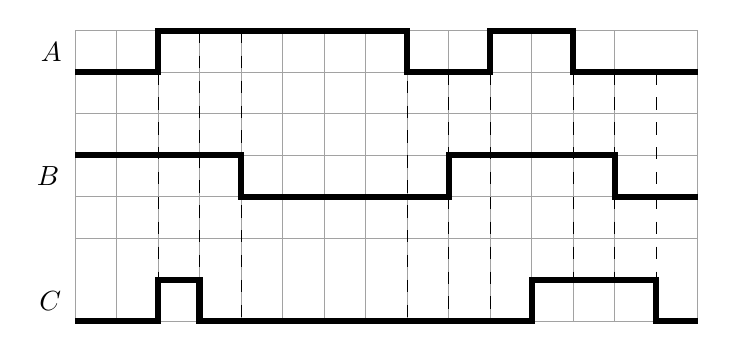
\begin{tikzpicture}[x=0.75pt,y=0.75pt,yscale=-1,xscale=1]
%uncomment if require: \path (0,300); %set diagram left start at 0, and has height of 300

%Shape: Grid [id:dp34531111101152123] 
\draw  [draw opacity=0] (100,40) -- (400,40) -- (400,180) -- (100,180) -- cycle ; \draw  [color={rgb, 255:red, 162; green, 162; blue, 162 }  ,draw opacity=1 ] (120,40) -- (120,180)(140,40) -- (140,180)(160,40) -- (160,180)(180,40) -- (180,180)(200,40) -- (200,180)(220,40) -- (220,180)(240,40) -- (240,180)(260,40) -- (260,180)(280,40) -- (280,180)(300,40) -- (300,180)(320,40) -- (320,180)(340,40) -- (340,180)(360,40) -- (360,180) ; \draw  [color={rgb, 255:red, 162; green, 162; blue, 162 }  ,draw opacity=1 ] (100,60) -- (400,60)(100,80) -- (400,80)(100,100) -- (400,100)(100,120) -- (400,120)(100,140) -- (400,140) ; \draw  [color={rgb, 255:red, 162; green, 162; blue, 162 }  ,draw opacity=1 ] (100,40) -- (400,40) -- (400,180) -- (100,180) -- cycle ;
%Straight Lines [id:da9908667716444586] 
\draw  [dash pattern={on 4.5pt off 4.5pt}]  (140,60) -- (140,160) ;


%Straight Lines [id:da9489034074703155] 
\draw  [dash pattern={on 4.5pt off 4.5pt}]  (160,40) -- (160,160) ;


%Straight Lines [id:da7444148673969375] 
\draw  [dash pattern={on 4.5pt off 4.5pt}]  (180,40) -- (180,180) ;


%Straight Lines [id:da33359589579811755] 
\draw  [dash pattern={on 4.5pt off 4.5pt}]  (260,40) -- (260,180) ;


%Straight Lines [id:da1689198722872045] 
\draw  [dash pattern={on 4.5pt off 4.5pt}]  (280,60) -- (280,180) ;


%Straight Lines [id:da2835936693187402] 
\draw  [dash pattern={on 4.5pt off 4.5pt}]  (300,60) -- (300,180) ;


%Straight Lines [id:da7069604701418795] 
\draw  [dash pattern={on 4.5pt off 4.5pt}]  (340,60) -- (340,160) ;


%Straight Lines [id:da35256438922338873] 
\draw  [dash pattern={on 4.5pt off 4.5pt}]  (360,60) -- (360,160) ;


%Straight Lines [id:da8396949759627998] 
\draw  [dash pattern={on 4.5pt off 4.5pt}]  (380,60) -- (380,160) ;


%Straight Lines [id:da8850959184881091] 
\draw [line width=2.25]    (100,60) -- (140,60) -- (140,40) -- (260,40) -- (260,60) -- (300,60) -- (300,40) -- (340,40) -- (340,60) -- (400,60) ;


%Straight Lines [id:da2574956876601695] 
\draw [line width=2.25]    (100,180) -- (140,180) -- (140,160) -- (160,160) -- (160,180) -- (320,180) -- (320,160) -- (380,160) -- (380,180) -- (400,180) ;


%Straight Lines [id:da8609754683162194] 
\draw [line width=2.25]    (100,100) -- (180,100) -- (180,120) -- (280,120) -- (280,100) -- (360,100) -- (360,120) -- (400,120) ;



% Text Node
\draw (88.5,50) node   {$A$};
% Text Node
\draw (87,110) node   {$B$};
% Text Node
\draw (88,170) node   {$C$};


\end{tikzpicture}
}
	
	Sinal em tempo contínuo e analógico
\end{minipage}\tikzmark{ar1}
\hfill
\begin{minipage}{0.48\linewidth}
	\centering
	
	\scalebox{0.5}{\deftkzbds
		
\begin{tikzpicture}[auto, node distance=2cm,>=Latex]
	% We start by placing the blocks
	\node [input] (input) {};
	\node [block, right=of input, xshift=0cm, align=center, text width=2cm] (computer) {$ h[n] $};
	\node [output, right =of computer] (output) {};
	\node [above, xshift=0.8cm] at (input) {$ x\left[n \right]  $};
	\node [above, xshift=-1cm] at (output) {$ y\left[n \right]  $};
	
	\draw [->] (input) -- (computer);
	\draw [->] (computer) -- (output);
\end{tikzpicture}}
	
	Sinal em tempo discreto e analógico
\end{minipage}

\begin{tikzpicture}[overlay, remember picture]
	\draw[-Implies, double distance=2pt] ($(ar1)+(-0.3,0)$) -- node[below] {\small Amostragem} +(0.8,0);
\end{tikzpicture}
	
\end{frame}


\begin{frame}{Sinais}
\begin{minipage}{0.48\linewidth}
	\centering
	
	\scalebox{0.5}{\deftkzbds
		
\begin{tikzpicture}[auto, node distance=2cm,>=Latex]
	% We start by placing the blocks
	\node [input] (input) {};
	\node [block, right=of input, xshift=0cm, align=center, text width=2cm] (computer) {$ h[n] $};
	\node [output, right =of computer] (output) {};
	\node [above, xshift=0.8cm] at (input) {$ x\left[n \right]  $};
	\node [above, xshift=-1cm] at (output) {$ y\left[n \right]  $};
	
	\draw [->] (input) -- (computer);
	\draw [->] (computer) -- (output);
\end{tikzpicture}}
	
	Sinal em tempo discreto e analógico
\end{minipage}\tikzmark{ar1}
\hfill
\begin{minipage}{0.48\linewidth}
	\centering
	
	\scalebox{0.51}{\deftkzbds

\begin{tikzpicture}[auto, node distance=2cm,>=Latex]
	% We start by placing the blocks
	\node [input] (input) {};
	\node [block, right=of input, xshift=0cm, align=center, text width=2cm] (computer) {$ h[n] $};
	\node [output, right =of computer] (output) {};
	\node [above, xshift=0.8cm] at (input) {$ z^{n} $};
	\node [above, xshift=-1cm] at (output) {$ H(z)z^{n} $};
	
	\draw [->] (input) -- (computer);
	\draw [->] (computer) -- (output);
\end{tikzpicture}}
	
	Sinal em tempo discreto e digital
\end{minipage}

\begin{tikzpicture}[overlay, remember picture]
\draw[-Implies, double distance=2pt] ($(ar1)+(-0.3,0)$) -- node[below] {Quantização} +(0.8,0);
\end{tikzpicture}

\bigskip

\begin{block}{Sinal digital}
\begin{itemize}
	\item Sinal \textbf{amostrado} no tempo.
	\item Sinal \textbf{quantizado} na amplitude.
\end{itemize}
\end{block}

\end{frame}


\begin{frame}{Malha de controle analógica}
	
	\centering
	
	\scalebox{0.8}{\begin{tikzpicture}[scale=1.5,>=latex, every node/.style={inner sep=2pt}]
	
	\draw[pattern=south east lines, draw=mWhite] (0cm,0cm) circle(1.4cm);

	\draw[dashed] (0cm,0cm) circle(1.4cm);

	\draw[dashed, fill=mWhite] (0cm,0cm) circle(0.6cm);
	
    % draw the coordinates
    \draw[->, fill=mWhite] (-2cm,0cm) -- (2cm,0cm) node[right=2pt,fill=mWhite] {$\Re(z)$};
    \draw[->, fill=mWhite] (0cm,-2cm) -- (0cm,2cm) node[above=2pt,fill=mWhite] {$\Im(z)$};
    
    \draw[fill=black] (-1.4,0) ++(-2pt,-2pt) -- ++(4pt,4pt) ++(-4pt,0pt) -- ++(4pt,-4pt) +(-2pt,2pt) node[below left=2pt] {$ -1,4 $};
    
%    \draw[fill=black] (-0.6,0) circle (1pt) node[below=2pt,fill=mWhite] {$ -0,6 $};
    
    \draw[fill=black] (0.6,0) ++(-2pt,-2pt) -- ++(4pt,4pt) ++(-4pt,0pt) -- ++(4pt,-4pt) +(-2pt,2pt) node[below left=2pt] {$ 0,6 $};
    
%    \draw[fill=black] (1.4,0) circle (1pt) node[below=2pt,fill=mWhite] {$ 1,4$};

%	\draw[->] (0,0) -- (45:1) node[left] {$ r=1 $};
\end{tikzpicture}}
	
	Sistema de controle em tempo contínuo
	
\end{frame}


\begin{frame}{Malha de controle digital}
	
	\centering
	
	\scalebox{0.65}{\deftkzbds
	
\begin{tikzpicture}[auto, node distance=2cm,>=Latex]
	
	\node [input, name=input] {};
	\node [sum, right =of input, xshift=0.5cm] (sum) {$\sum$};
	\node [block, right =of sum, text width=2cm, align=center] (computer) {Computador digital};
	
	\node [block, right=of computer] (DA) {D/A};
	\draw [->] (computer) -- node[name=uk] {$u(kT)$} (DA);
	\node [block, right =of DA, pin={[pinstyle]above:$w(t)$},
	node distance=3cm] (process) {Planta};
	\node[below=20pt, circle, draw] at (process) {\Large 1};
	\draw [->] (DA) -- node[name=u] {$u(t)$} (process);
	% We draw an edge between the computer and process block to 
	% calculate the coordinate u. We need it to place the measurement block. 
	\node [output, right =of process] (output) {};
	
	\node [block, below=of computer, yshift=2cm, xshift=1.4em, minimum width=4em] (clock) {Clock};
	
	\node [block, below =of DA, pin={[pinstyle]below:$v(t)$}, yshift=-0.5cm] (sensor) {Sensor};
	\node [block, left=4cm] at (sensor) (AD) {A/D};
	\node[below=20pt, circle, draw] at (AD) {\Large 2};
	
	\draw [->] (clock) -| (DA);
	\draw [->] (clock) -| (AD);
	
	\draw [draw,->] (input) -- node {$r(kT)$} (sum);
	\draw [->] (sum) -- node {$\hat{e}(kT)$} (computer);
	\draw [->] (process) -- node [name=y] {$y(t)$}(output);
	\draw [->] (y) |- (sensor);
	\draw [->] (sensor) -- node[yshift=15pt] {$\hat{y}(t)$} (AD);
	\draw [->] (AD) -| node[pos=0.98, xshift=15pt] {$-$} node[pos=1.15, xshift=-4pt] {$+$} node [near start, yshift=15pt] {$\hat{y}(kT)$} (sum);
\end{tikzpicture}}
	
	Sistema de controle digital (a lei de controle é implementada em um computador digital)
	
\end{frame}

\begin{frame}{Malha de controle digital}
\begin{block}{Sistema de controle digital}
\begin{itemize}
	\item $ r \rightarrow$ entrada de referência
	\item $ u \rightarrow$ sinal de controle
	\item $ y \rightarrow$ sinal de saída
	\item $ \hat{y} \rightarrow$ sinal de saída estimado
	\item $ \hat{e}=r-\hat{y} \rightarrow$ erro do sistema
	\item $ w \rightarrow$ entrada de distúrbio na planta
	\item $ v \rightarrow$ ruído de entrada no sensor
	\item A/D $ \rightarrow$ conversor analógico para digital
	\item D/A $ \rightarrow$ conversor digital para analógico
\end{itemize}
\end{block}
\end{frame}

\begin{frame}{Malha de controle digital}
\begin{block}{Descrição dos componentes da malha}
\begin{enumerate}
	\item A planta é o processo a ser controlado, que necessita de um controle para alcançar uma \textbf{resposta satisfatória} mesmo na $ \underbrace{\text{presença de distúrbios}}_{\text{rejeição a distúrbios}} $ $ w(t) $ e ruídos $ v(t) $.
\end{enumerate}

\vspace{0.5cm}

\begin{itemize}
	\item $ y(t)\to r(t) $: \textbf{regulação} (resposta satisfatória).
	\item Controle/sistema robusto $\rightarrow$ baixa sensibilidade a mudanças de parâmetros da planta $ + $ rejeição a distúrbios.
\end{itemize}
\end{block}
\end{frame}


\begin{frame}{Malha de controle digital}
\begin{block}{Descrição dos componentes da malha}
\begin{enumerate}
	\setcounter{enumi}{1}
	\item A/D: O conversor faz a leitura do sinal vindo do sensor, normalmente em tensão, e converte em uma sequência de números.
\end{enumerate}

\vspace{0.5cm}

\begin{itemize}
	\item Pode haver um erro $ \hat{y} $ no processo de computação.
	\item Assume-se que os sinais são amostrados em um período fixo $ T $ \textbf{(tempo de amostragem)}.
\end{itemize}
\end{block}
\end{frame}


\begin{frame}{Malha de controle digital}

\scalebox{0.75}{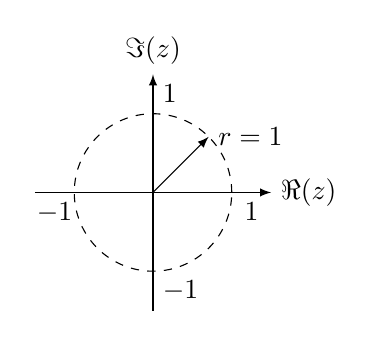
\begin{tikzpicture}[scale=1,>=latex]
        % draw the coordinates
        \draw[->] (-1.5cm,0cm) -- (1.5cm,0cm) node[right,fill=white] {$\Re(z)$};
        \draw[->] (0cm,-1.5cm) -- (0cm,1.5cm) node[above,fill=white] {$\Im(z)$};

        % draw the unit circle
        \draw[dashed] (0cm,0cm) circle(1cm);
        
        \draw[->] (0,0) -- (45:1) node[right] {$ r=1 $};

        % draw the horizontal and vertical coordinates
        % the placement is better this way
        \draw (-1.25cm,0cm) node[below] {$ -1 $}
              (1.25cm,0cm)  node[below] {$ 1 $}
              (0cm,-1.25cm) node[right] {$ -1 $}
              (0cm,1.25cm)  node[right] {$ 1 $};
    \end{tikzpicture}}

\vspace{0.5cm}

\begin{block}{Observação}
\begin{itemize}
	\item Para $ T $ e $ q $ pequenos, sinais digitais são “praticamente contínuos”.
\end{itemize}
\end{block}

\end{frame}

\begin{frame}{Malha de controle digital}

\begin{block}{Quantização}
Após a discretização, ou amostragem do sinal, é realizada a \textbf{quantização}. O sinal é
convertido numa \textbf{sequência binária} para ser lido pelo computador, onde o valor será truncado para o número mais próximo representável pelo computador.
\end{block}

\vspace{0.2cm}

\centerline{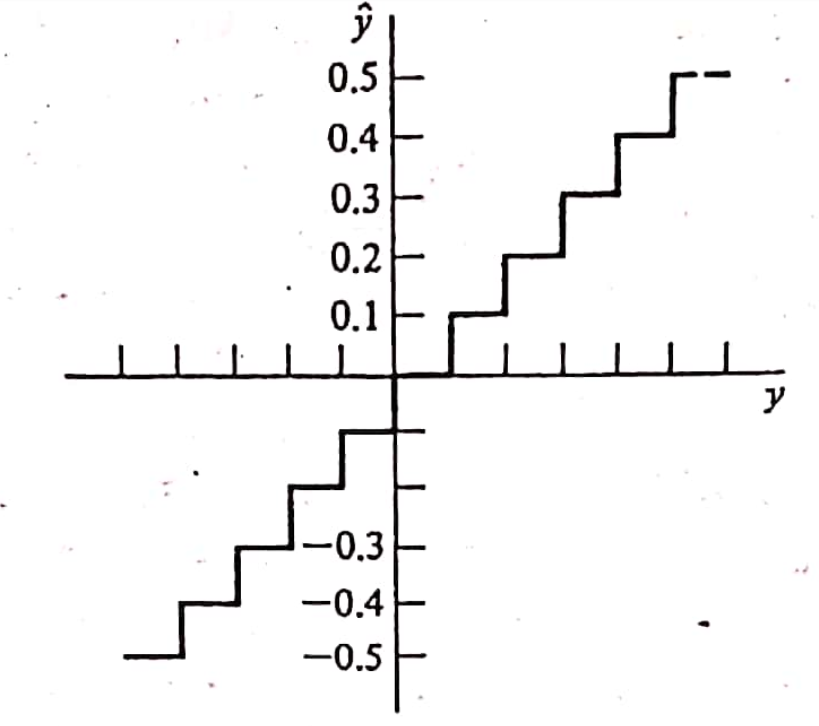
\includegraphics[width=0.4\linewidth]{Figuras/Ch01/fig2.PNG}}

\end{frame}

\begin{frame}{Malha de controle digital}

\begin{block}{Exemplo}
\begin{itemize}
    \item Controle digital de temperatura
\end{itemize}
\end{block}

\centerline{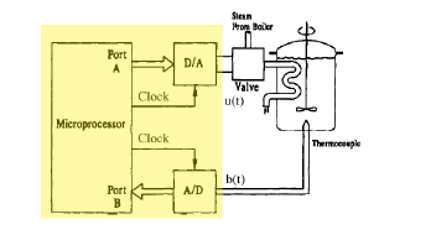
\includegraphics[width=0.9\linewidth]{Figuras/Ch01/fig1.png}}

\end{frame}

\begin{frame}{Técnicas de projeto}
\begin{block}{}
\begin{enumerate}
\item Projetar em $ s \rightarrow $ converter para $ z $.
\item Projetar diretamente em $ z $.
\end{enumerate}
\end{block}
	
	
\end{frame}

\begin{frame}{“Maldições” do controle digital }
\begin{block}{}
\begin{enumerate}
		\item \textbf{Amostrado} no tempo.
		\item \textbf{Quantizado} em amplitude.
		\item \textbf{Atrasado} no tempo $ \rightarrow $ efeito \tikzmark{t1}do D/A $ \rightarrow $ \textbf{ZOH}.
	\end{enumerate}
	
	\begin{tikzpicture}[auto, node distance=0.5cm, overlay, remember picture]
	
	\node(t2) [below=of t1, yshift=-5pt] {atraso de $ \dfrac{T}{2}\,\si{\second} $};
	
	\node (t3) [below= of t2] {$ G_H(s)=\text{e}^{-sT/2} $};
	
	\draw[->] ($(t1)+(0,-5pt)$) -- (t2);
	\draw[->] (t2) -- (t3);
	
	\end{tikzpicture}
	
	\vspace{2.8cm}
	
	\begin{itemize}
		\item \textbf{Aproximação de Padé:} $ H(s)=\dfrac{2/T}{s+2/T} $
		\item \MATLAB
	\end{itemize}
\end{block}
\end{frame}

\begin{frame}{Vantagens x Desvantagens}
\begin{block}{Vantagens}
\begin{itemize}
	\item Fácil para implementar as leis de controle.
	\item Fácil para mudar as leis de controle.
	\item Menor sensibilidade à ruídos.
	\item Menor sensibilidade à desgaste de componentes.
	\item Menor.
	\item Mais leve.
	\item Custo cada vez mais baixo.
\end{itemize}
\end{block}
\end{frame}

\begin{frame}{Vantagens x Desvantagens}
\begin{block}{Desvantagens}
\begin{itemize}
	\item Banda limitada (taxa de amostragem).
	\item Resolução.
	\item Velocidade de computação.
\end{itemize}
\end{block}
\end{frame}

\begin{frame}{Nomenclatura}
\begin{block}{Variáveis}
\begin{itemize}
	\item \textbf{Tempo contínuo}: $m(t)$ será considerada de tempo contínuo, pois $t \in \mathbb{R}$, ou seja, para qualquer valor de tempo $t$, $m(t)$ é definida.
	\item \textbf{Tempo discreto}: se $m(t)$ for conhecida apenas em instantes específicos de tempo $t_1, t_2, t_3 ...$ em que $t_n \in \mathbb{R}$ dizemos que a sequência de valores $m(t_n)$ é um sinal de tempo discreto. 
\end{itemize}
\end{block}
\end{frame}

\begin{frame}{Nomenclatura}
\begin{block}{Período de amostragem}
\begin{itemize}
	\item  Se os instantes $t_n$ estiverem \textbf{igualmente espaçados no tempo}, ou seja, se $T = t_n - t_{n-1}$, $n\in \mathbb{Z}$, podemos escrever $t_1 = T$, $t_2 = 2T$, $t_3 = 3T$ ... em que $T \in \mathbb{R}$ é um valor constante chamado de \textbf{período de amostragem} e o sinal amostrado pode ser representado como $m(nT)$ ou simplesmente $m(k)$, $k\in \mathbb{Z}$.
	\item A diferença entre as representações $m(nT)$ e $m(k)$ é sutil, mas relevante. Note que o domínio de $m(nT)$ é real e tem unidade de tempo, ao passo que $m(k)$ está representado no domínio de amostras ou observações, que é inteiro e adimensional.
\end{itemize}
\end{block}
\centerline{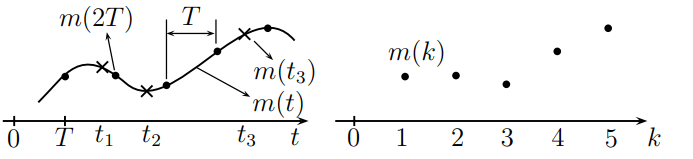
\includegraphics[width=0.9\linewidth]{Figuras/Ch01/fig3.PNG}}
\end{frame}

\begin{frame}{Sinais elementares}
\begin{block}{Função degrau unitário contínuo (\textit{função de Heavside})}
\begin{equation*}
u(t) = \begin{cases}
0, & \forall t < 0 \\
1, & \forall t \geq 0
\end{cases}
\end{equation*}
\end{block}
\centerline{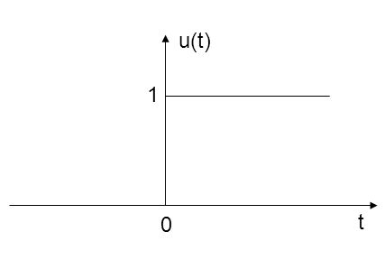
\includegraphics[width=0.5\linewidth]{Figuras/Ch01/fig4.PNG}}
\end{frame}

\begin{frame}{Sinais elementares}
\begin{block}{Função degrau unitário contínuo transladado}
\begin{equation*}
u(t - t_0) = \begin{cases}
0, & \forall t < t_0 \\
1, & \forall t \geq t_0
\end{cases}
\end{equation*}
\end{block}
\centerline{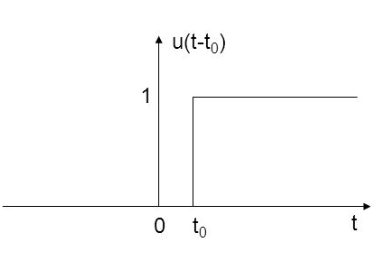
\includegraphics[width=0.5\linewidth]{Figuras/Ch01/fig5.PNG}}
\end{frame}

\begin{frame}{Sinais elementares}
\begin{block}{Função degrau unitário discreto (\textit{função de Heavside})}
\begin{equation*}
u(n) = \begin{cases}
0, & \forall n < 0 \\
1, & \forall n \geq 0
\end{cases}
\end{equation*}
\end{block}
\centerline{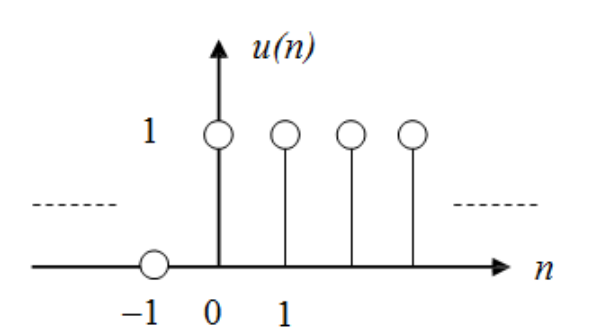
\includegraphics[width=0.5\linewidth]{Figuras/Ch01/fig6.PNG}}
\end{frame}

\begin{frame}{Sinais elementares}
\begin{block}{Função degrau unitário discreto transladado}
\begin{equation*}
u(n - k) = \begin{cases}
0, & \forall n < k \\
1, & \forall n \geq k
\end{cases}
\end{equation*}
\end{block}
\centerline{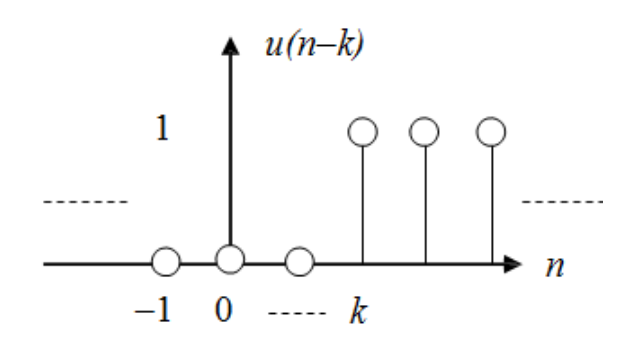
\includegraphics[width=0.5\linewidth]{Figuras/Ch01/fig7.PNG}}
\end{frame}

\begin{frame}{Sinais elementares}
\begin{block}{Função sinc}
\begin{equation*}
\text{sinc}(\theta) = \dfrac{\text{sen} \ \pi \theta}{\pi \theta}
\end{equation*}
\end{block}
\centerline{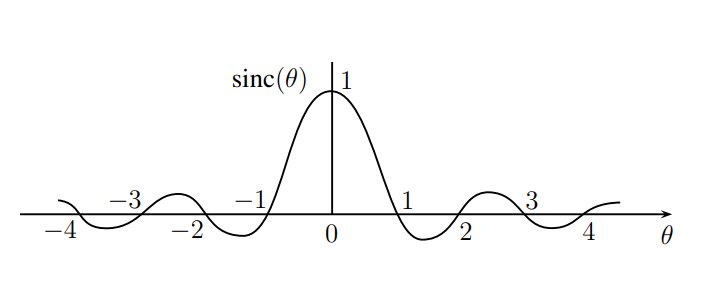
\includegraphics[width=0.9\linewidth]{Figuras/Ch01/fig8.PNG}}
\end{frame}

\begin{frame}{Sinais elementares}
\begin{block}{Função impulso unitário contínuo (\textit{delta de Dirac})}
\vspace{0.2cm}
\begin{align*}
    \delta (t) & = 0, \quad \forall t \neq 0 \\
    1 & = \int_{-\infty}^{+\infty} \delta (t) \ dt
\end{align*}
\begin{itemize}
    \item O fato de $\delta(t)$ ser \textbf{infinito} para $t = 0$ é indicado no gráfico pela seta. 
    \item Portanto, para $t = 0$ não faz sentido falar da “amplitude” do impulso, mas como a integral é finita, fala-se em \textbf{peso}.
\end{itemize}
\end{block}
\centerline{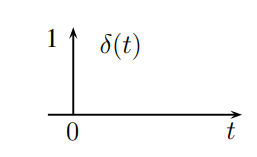
\includegraphics[width=0.4\linewidth]{Figuras/Ch01/fig9.PNG}}
\end{frame}

\begin{frame}{Sinais elementares}
\begin{block}{Função impulso unitário discreto (\textit{delta de Kronecker})}
\begin{equation*}
\delta(n) = \begin{cases}
0, & \forall n \neq 0 \\
1, & \forall n = 0
\end{cases}
\end{equation*}
\end{block}
\vspace{0.2cm}
\centerline{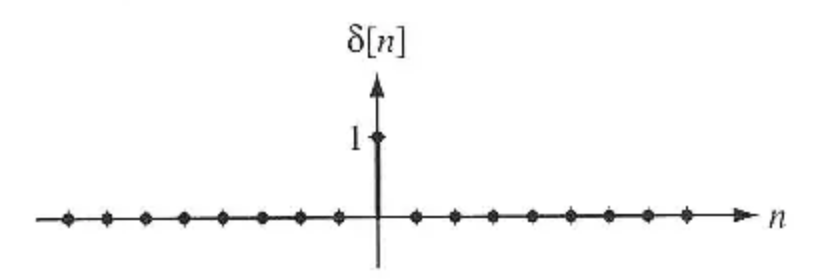
\includegraphics[width=0.8\linewidth]{Figuras/Ch01/fig10.PNG}}
\end{frame}

\frame{
\frametitle{Exercícios}
\begin{block}{}
01. Como expressar matematicamente a função impulso unitário discreto em termos da função degrau unitário discreto e vice-versa?

\vspace{1cm}

02. Explique a distinção entre um sistema de controle discreto, um digital e um sistema de controle amostrado.

\vspace{1cm}

03. Seja $m(t)$ um sinal contínuo qualquer e as constantes: $t_n, T \in \mathbb{R}$; $n, k \in \mathbb{Z}$. Discuta as semelhanças e diferenças dos seguintes sinais: $m(t)$, $m(t_n)$, $m(nT)$ e $m(k)$.
\end{block}
}

\frame{
\frametitle{Referências e exercícios complementares}
\begin{itemize}
\item AGUIRRE, Luis A. Controle de Sistemas Amostrados, 1 ed. [s.n.], 2019.
\end{itemize}
\centering{\alert{Página 25 - \textbf{Capítulo 1}}} \\
\vspace{0.4cm}
\begin{itemize}
\item FRANKLIN, Gene F.; POWELL, J. David; WOLKMAN, Michael L. Digital Control of Dynamic Systems, 3 ed. Addison-Wesley, 1998.
\end{itemize}
\centering{\alert{Página 8 - \textbf{Capítulo 1}}} \\
}

